%!TEX program = xelatex
% Note: this template must be compiled with XeLaTeX rather than PDFLaTeX
% due to the custom fonts used. The line above should ensure this happens
% automatically, but if it doesn't, your LaTeX editor should have a simple toggle
% to switch to using XeLaTeX.

\documentclass[
  aspectratio=169, % Uncomment to use an aspect ratio of 16:9 (160 mm by 90 mm)
  %aspectratio=43, % Uncomment to use an aspect ratio of 4:3 (128mm by 96mm)
  t, % Top align all slide content by default
  onlytextwidth, % Typeset content in columns at text width
  10pt, % Default font size, use 10pt for the 16:9 aspect ratio and 8pt for the 4:3 aspect ratio
]{beamer}

\usepackage{../../ImperialTheme/beamer/beamerthemeImperial} % Use the Imperial theme
\usepackage{xcolor}

\definecolor{tabpurple}{RGB}{148, 103, 189}
\definecolor{tabcyan}{RGB}{23, 190, 207}
\definecolor{tabred}{RGB}{214, 39, 40}

\def\imagefolder{../../ImperialTheme/beamer/Images}
\def\Rey{\text{Re}}
\title{Re analysis} % Presentation title to appear on the title slide and left footers

\subtitle{} % Presentation subtitle to appear on the title slide

\author{Víctor Ballester} % Author name(s) to appear on the title slide

\date{\today} % Presentation date to appear on the title slide and right footers

\begin{document}

\begingroup
\setbeamercolor{background canvas}{bg=ICLLightGrey} % Slide background color
\setbeamercolor{title page title}{fg=ICLBlue} % Title text color
\setbeamercolor{title page subtitle}{fg=ICLBlue} % Subtitle text color
\setbeamercolor{author}{fg=ICLBlue} % Author(s) text color
\setbeamercolor{date}{fg=ICLBlue} % Date text color
\setbeamertemplate{title page}[logo]{\imagefolder/ICL_Logo_Blue.pdf} % Imperial logo color, use 'ICL_Logo_White.pdf' for white and 'ICL_Logo_Blue.pdf' for blue
\frame[plain, s]{\titlepage} % Output the title page with no footer ('plain') and vertically distributed text ('s')
\endgroup

\begin{frame}
	\frametitle{Transition starting from 3d mode}
	I start the simulation with the baseflow and 3d mode. And the small noise of the mesh and 3d mose is enough to trigger the transition.
	\begin{figure}[ht]
		\centering
		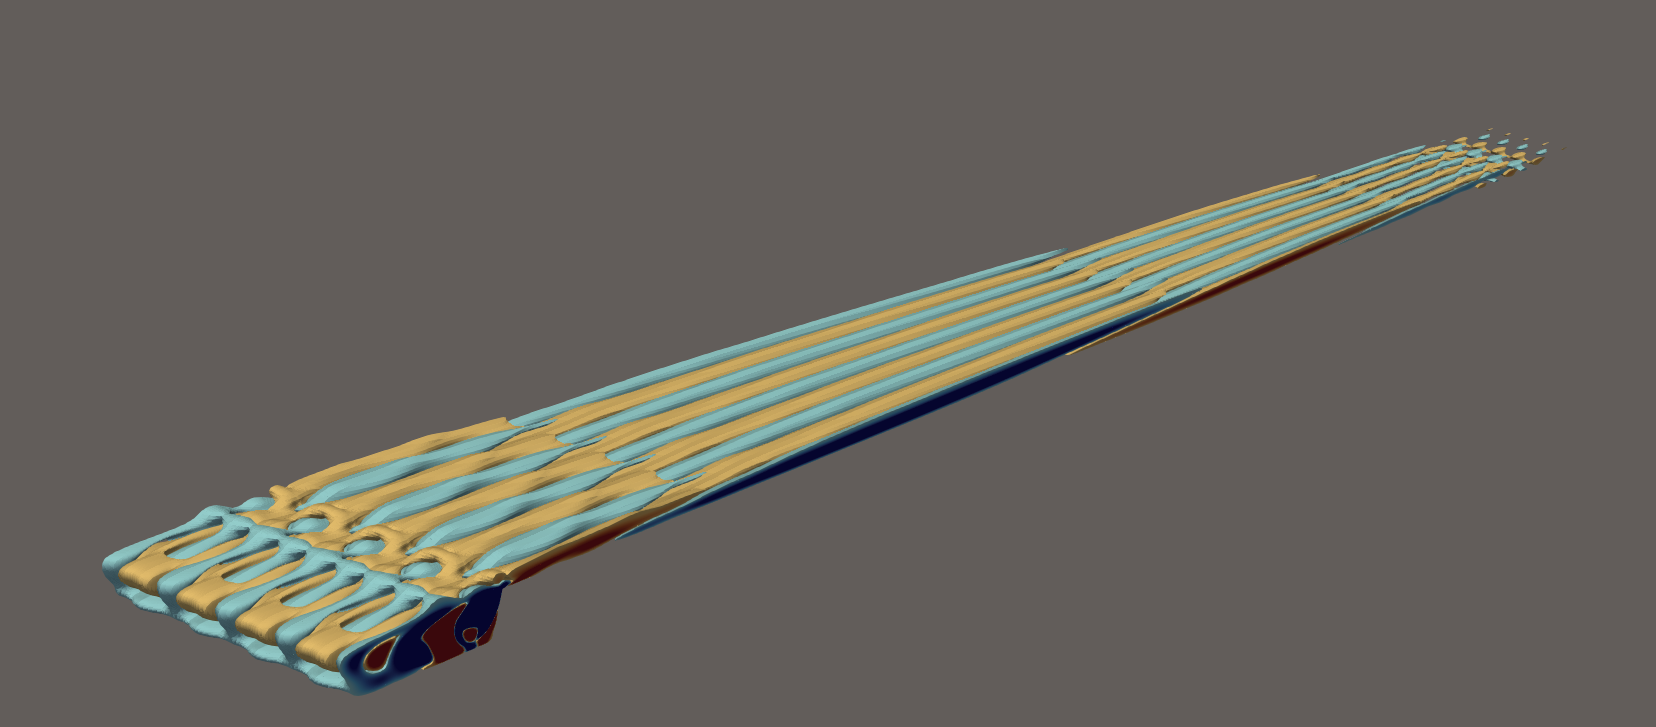
\includegraphics[width=0.9\textwidth]{Images/trans14.png}
	\end{figure}
\end{frame}
\begin{frame}
	\begin{figure}[ht]
		\centering
		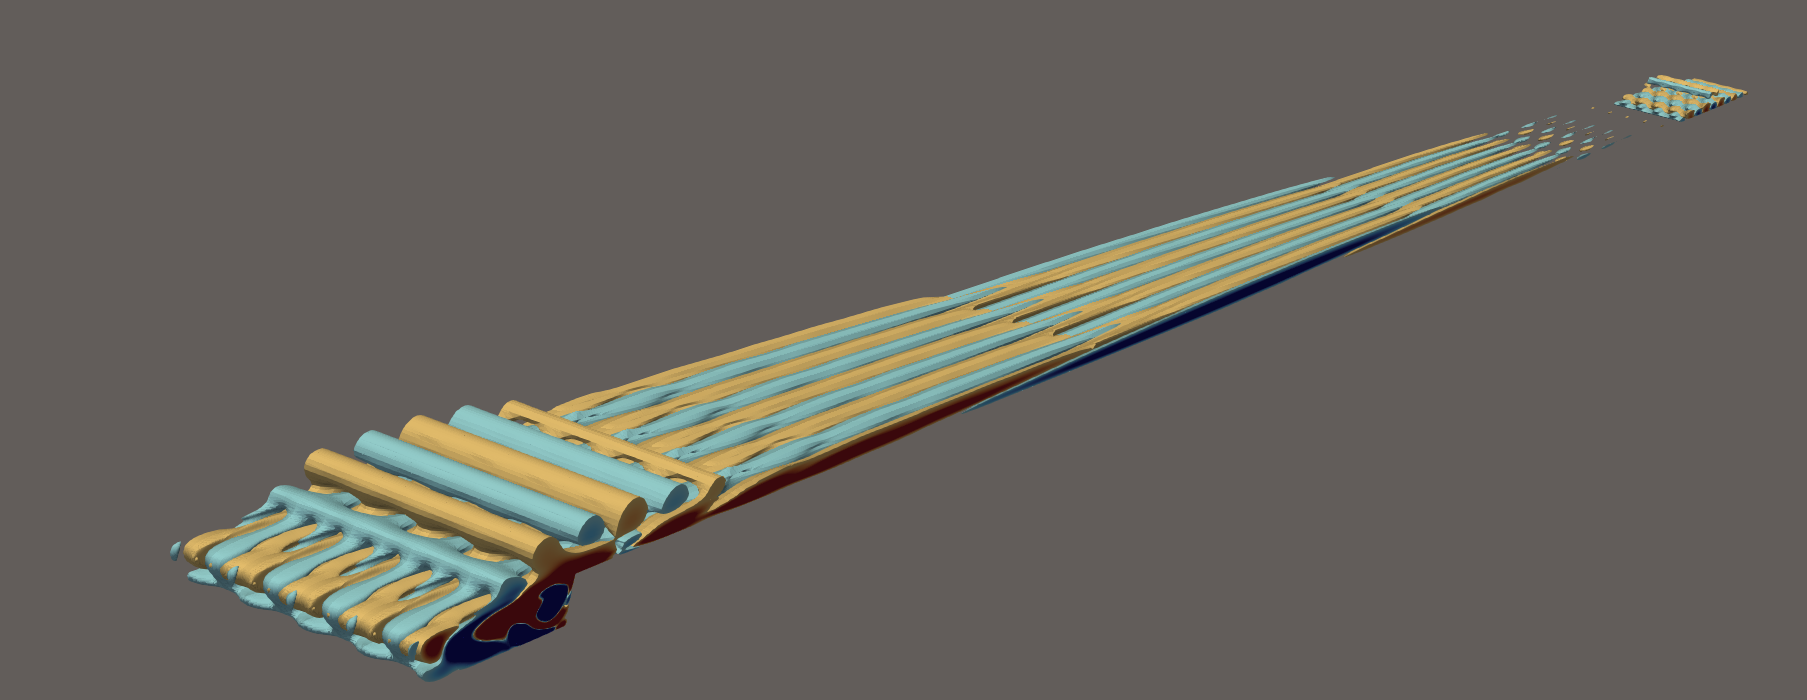
\includegraphics[width=\textwidth]{Images/trans16.png}
	\end{figure}
\end{frame}
\begin{frame}
	\begin{figure}[ht]
		\centering
		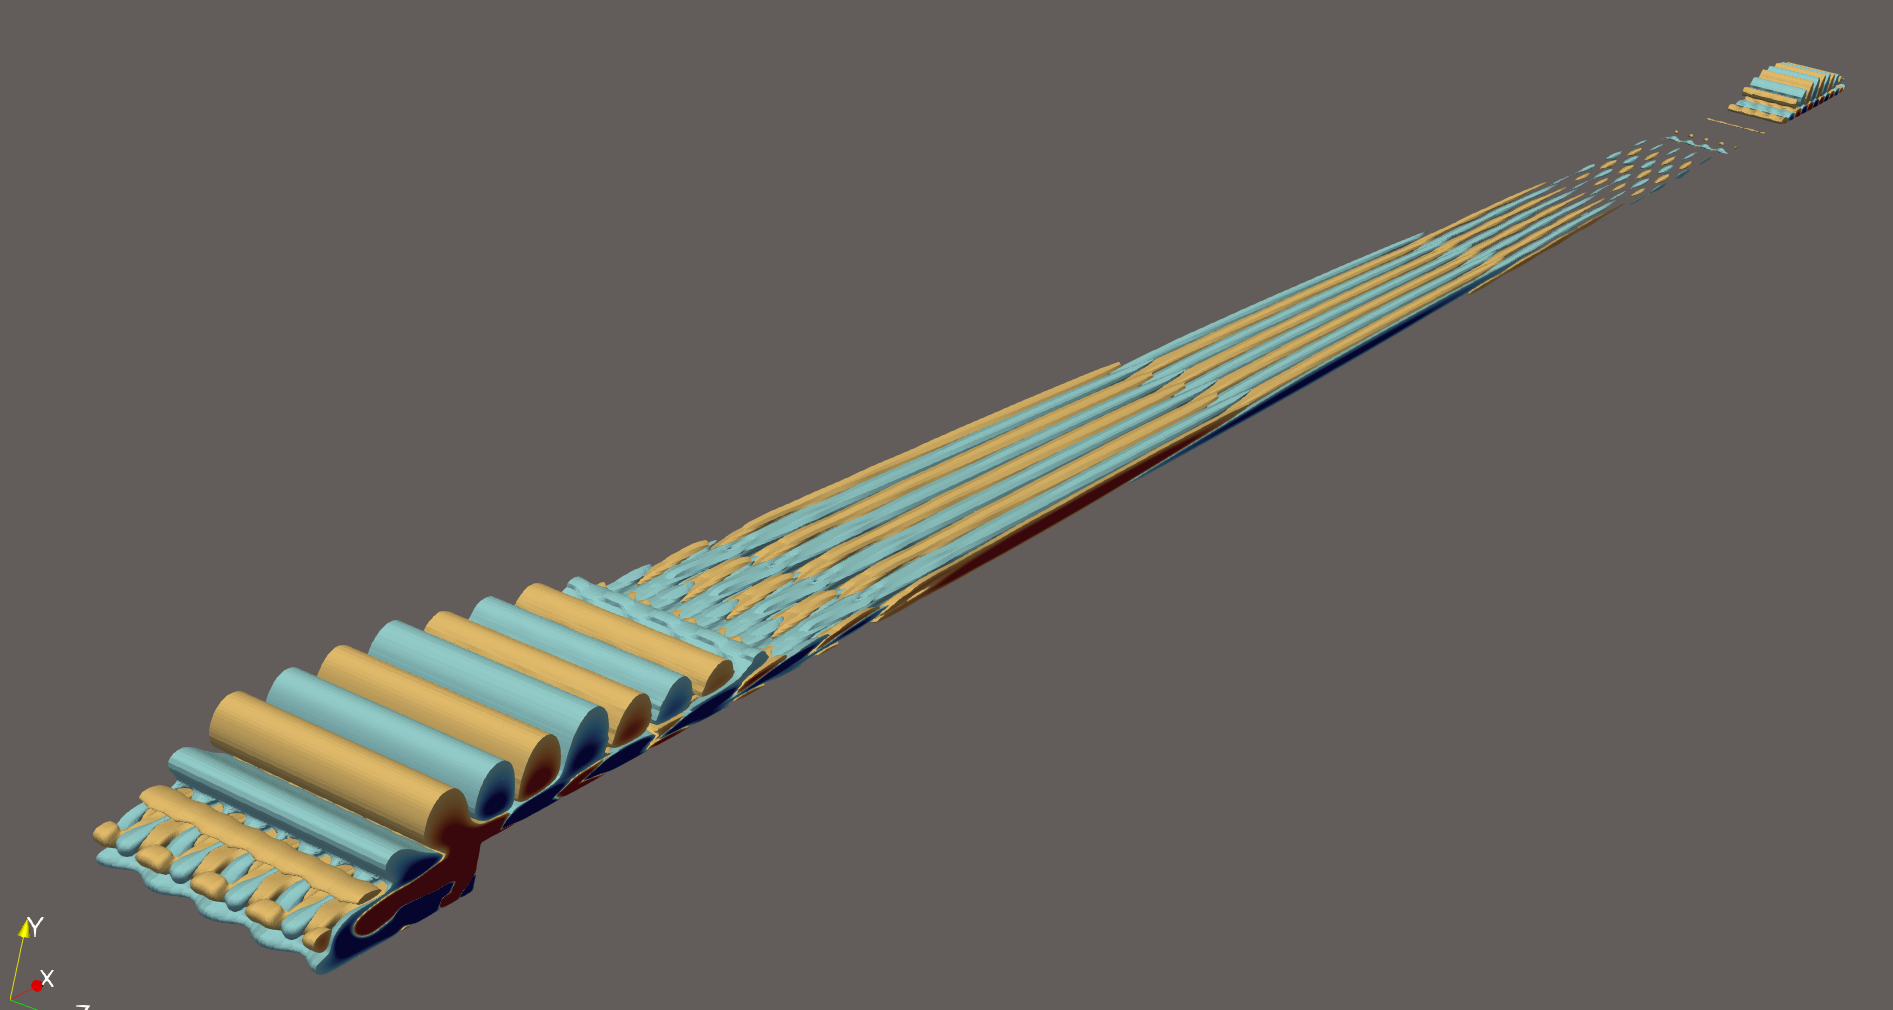
\includegraphics[width=\textwidth]{Images/trans18.png}
	\end{figure}
\end{frame}
\begin{frame}
	\begin{figure}[ht]
		\centering
		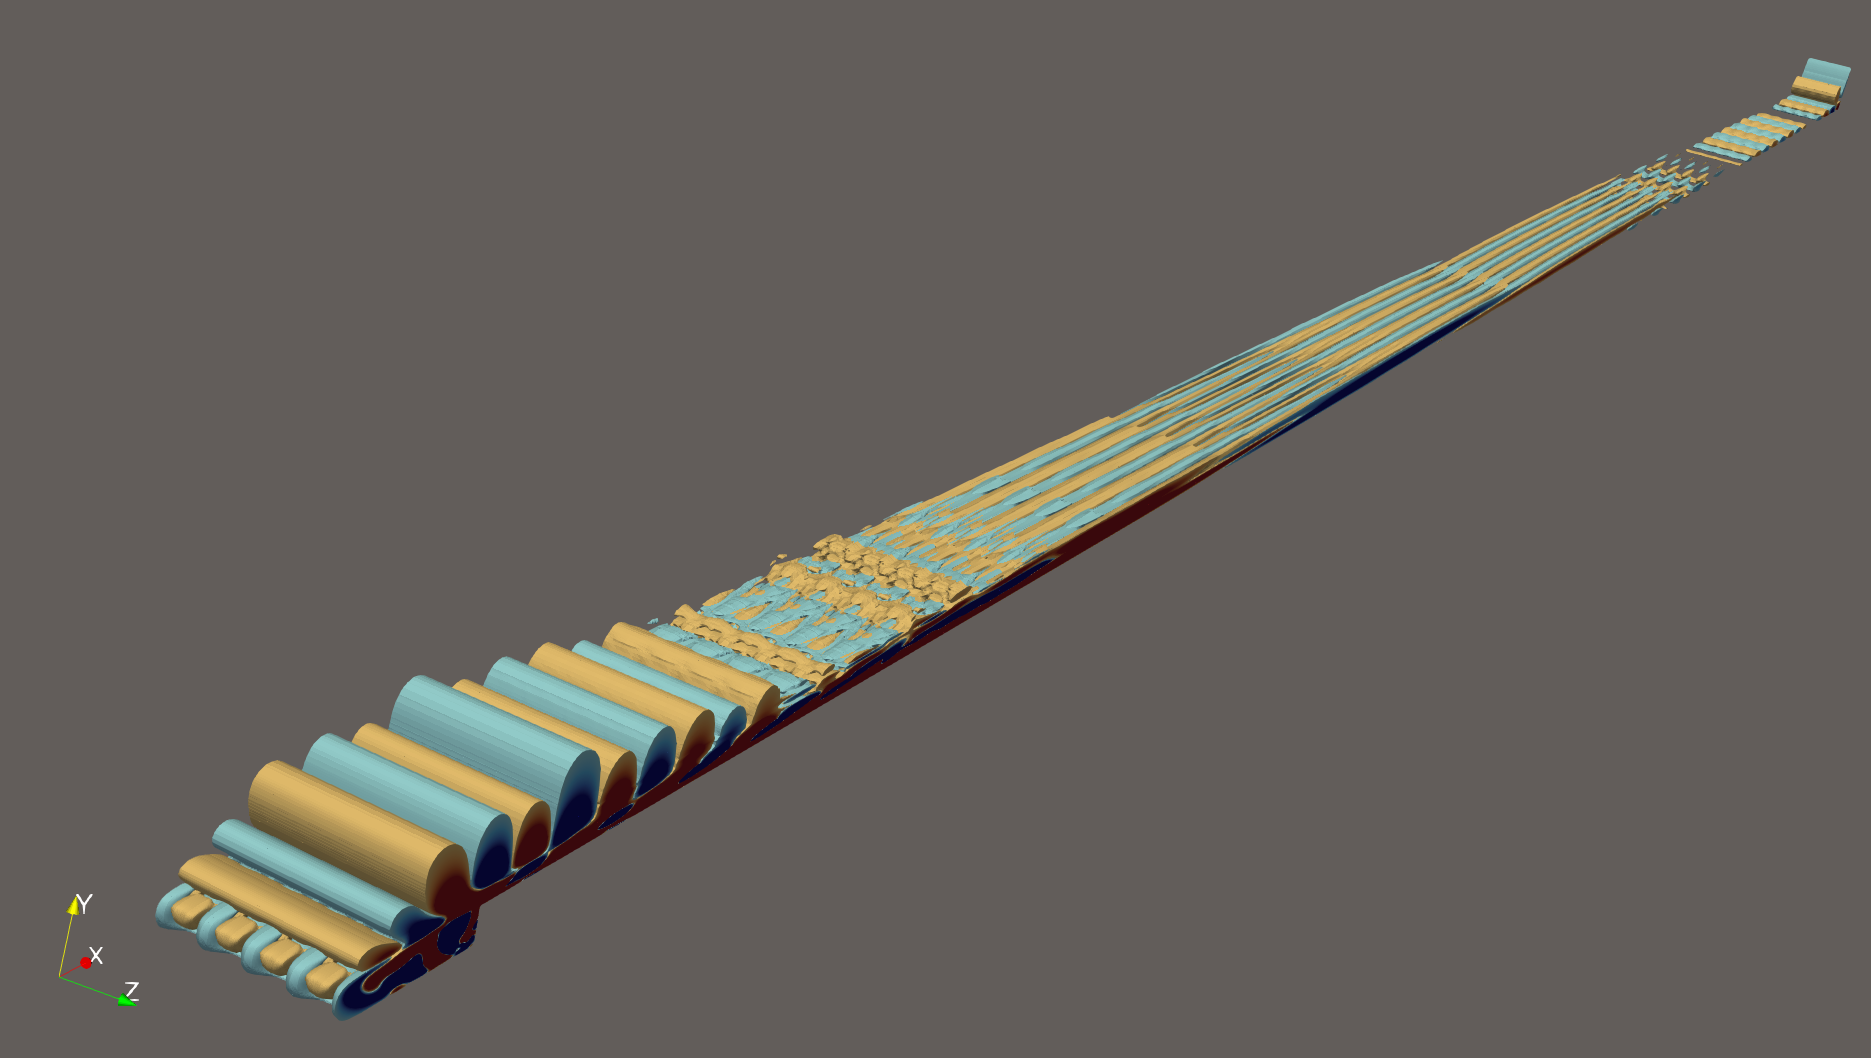
\includegraphics[width=\textwidth]{Images/trans20.png}
	\end{figure}
\end{frame}
\begin{frame}
	\frametitle{secondary bifurcation in 2d dynamics}
	\begin{itemize}
		\item When I run floquet analyis (with respect to the non-linear stable P.O.) I find two modes. The first one is the one that evolves to the P.O. that I linearized about (the nonlinear period is slighlty different from the linear one). The second mode is a new mode.
		\item freq mode 1: $\omega_1 = 0.174$ (frequency of the P.O. I linearize around is $\omega = 0.169$)
		\item freq mode 2: $\omega_2 = 0.216$
		\item I don't know whether the difference $\omega_2 - \omega_1$ is related to $\simeq 1/3\omega_1$, which is what I observed on the time periodic signals around the bifurcation point.
	\end{itemize}
\end{frame}
\begin{frame}
  	\begin{columns}[T] % [T] ensures correct vertical alignment
		\begin{column}{0.495\linewidth} % left column
			\begin{figure}[ht]
				\centering
				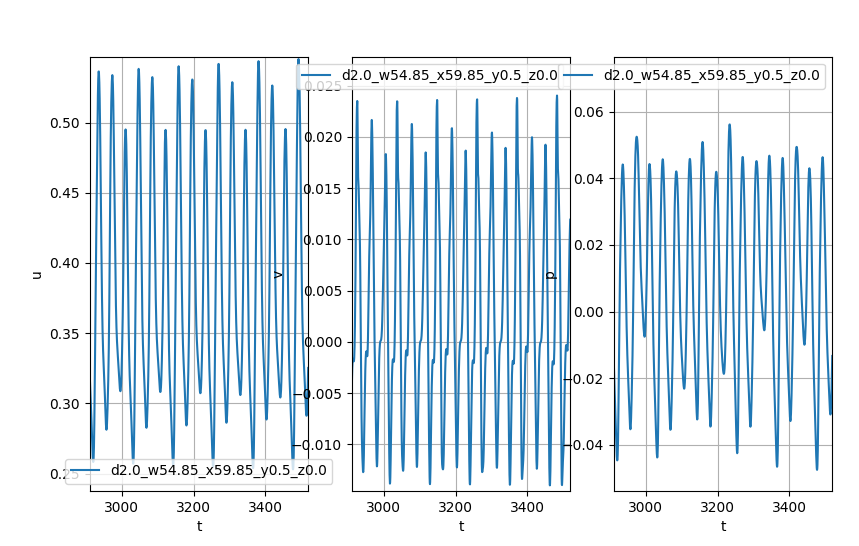
\includegraphics[width=\linewidth]{Images/unstableTimeseries.png}
			\end{figure}
			Time series destabilising when starting around the periodic orbit (showing the 3T period)
		\end{column}
		\begin{column}{0.495\linewidth} % left column
			\begin{figure}[ht]
				\centering
				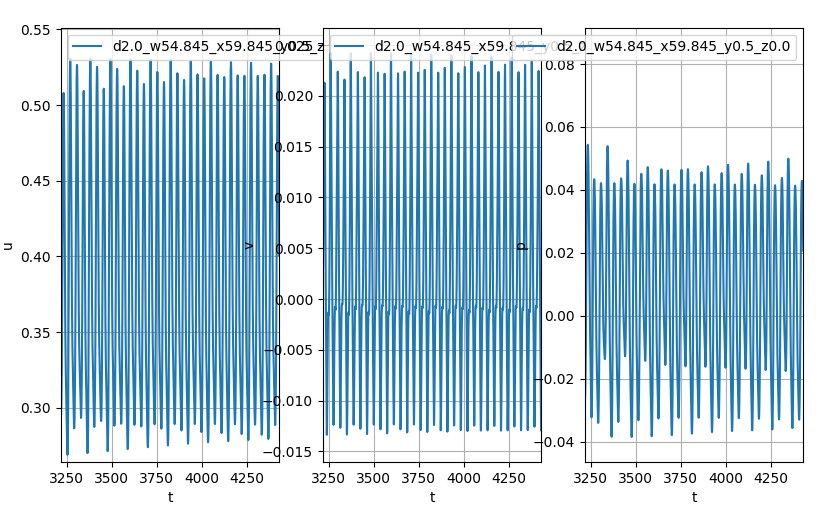
\includegraphics[width=\linewidth]{Images/stableTimeseries.png}
			\end{figure}
			Time series stabilising when starting around the periodic orbit (showing the 3T period stabilizing to the 1T period)
		\end{column}
	\end{columns}
\end{frame}
\end{document}
